\begin{section}{Zwangsläufigkeit}
  Dieser Abschnitt widmet sich dem Beweis von Satz \ref{2.3}.
 
 \begin{definition}{Wagenrad, Radnabe}
  Eine Konfiguration $W$ heißt \textit{Wagenrad} (engl.: cartwheel), wenn es einen Knoten $w$, genannt \textit{Radnabe} (engl.: hub), und zwei Kreise $C_1, C_2$ mit folgenden Eigenschaften gibt:
  \begin{enumerate}[(i)]
   \item es gilt $\{w\} \cap C_1 = \emptyset,\{w\} \cap C_2 = \emptyset$ und $C_2 \cap C_1 = \emptyset$, aber $\{w\} \cup C_1 \cup C_2 = V(G(W))$,
   \item $C_1$ und $C_2$ sind Teilgraphen von $G(W)$ und die Außenfacette von $C_2$ ist die Außenfacette von $G(W)$,
   \item $w$ ist adjazent zu allen Knoten von $C_1$ aber keinem Knoten von $C_2$.
  \end{enumerate}
 \end{definition}

 Es gibt folglich also vier Sorten von Kanten in einem Wagenrad: Kanten von $C_1$, Kanten von $C_2$, Kanten zwischen $w$ und und $C_1$ sowie Kanten zwischen $C_1$ und $C_2$. Zur Veranschaulichung noch eine Darstellung eines Wagenrades.
 
 \begin{figure}[ht]
  \label{fig3}
  \[ \begin{tikzpicture}
 \draw
    (0,1.5) \smallnode(a1){} (0,2) \rectanglenode(a2){} (0,4) \blacknode(a3){}
    (0.5,1) \smallnode(b1){}
    (1,0.5) \smallnode(c1){} (1,3) \blacknode(c2){}
    (2,0) \smallnode(d1){} (2,1.5) \rectanglenode(d2){} (2,5) \blacknode(d3){} (2,6) \rectanglenode(d4){} 
    (3,1) \blacknode(e1){} (3,3) \rectanglenode(e2){w} (3,5.5) \blacknode(e3){} 
    (4,0) \smallnode(f1){} (4,1.5) \smallnode(f2){} (4,5) \blacknode(f3){} (4,6) \blacknode(f4){} 
    (5,3) \whitenode(g1){} (5,5) \rectanglenode(g2){}
    (5.5,1) \whitenode(h1){} 
    (6,2) \smallnode(i1){} (6,3) \smallnode(i2){} (6,4) \smallnode(i3){};
    \filldraw (a1) -- (b1) -- (c1) -- (d1) -- (f1) -- (h1) -- (i1) -- (i2) -- (i3) -- (g2) -- (f4) -- (d4) -- (a3) -- (a2) -- (a1);
    \filldraw (c2) -- (d2) -- (e1) -- (f2) -- (g1) -- (f3) -- (e3) -- (d3) -- (c2) -- (e2) -- (g1);
    \filldraw (e1) -- (e2) -- (e3);
    \filldraw (f3) -- (e2) -- (d2) -- (d1) -- (e1) -- (f1) -- (f2) -- (e2) -- (d3);
    \filldraw (b1) -- (d2) -- (c1);
    \filldraw (a1) -- (d2) -- (a2) -- (c2) -- (a3) -- (d3) -- (d4) -- (e3) -- (f4) -- (f3) -- (g2) -- (g1) -- (i3);
    \filldraw (i2) -- (g1) -- (i1) -- (f2) -- (h1);
\end{tikzpicture}     \]
  \caption[Darstellung eines Wagenrads]{Darstellung eines Wagenrads}
 \end{figure}

 Die folgende Proposition geht zurück auf Birkhoff, genauer nachzulesen in \cite{AmJMath35}.
 
 \begin{propositionl}{Eindeutiges Wagenrad}{4.1}
  Sei $T$ eine intern 6-fach zusammenhängende Triangulation und sei $w$ ein Knoten von $T$. Dann gibt es in $T$ genau ein Wagenrad mit Radnabe $w$.
 \end{propositionl}
 
 \begin{definition}{Auftretendes Wagenrad}
  Sei $W$ ein Wagenrad. Eine Konfiguration $K$ \textit{tritt in $W$ auf}, wenn $G(K)$ eine Teilzeichnung von $G(W)$ ist, jede Innenfacette von $K$ eine Innenfacette von $W$ ist und $\gamma_K(v) = \gamma_W(v)$ für alle $v\in V(G(K))$ gilt. 
 \end{definition}
 
 \begin{definition}{Fluss, Wert, Quelle, Senke, $N_\itP(W)$, $\mathscr{W}_T$}
  Ein \textit{Fluss} $P$ (engl.: pass) ist ein 4-Tupel $(K,r,s,t)$ mit
  \begin{itemize}
   \item einer Konfiguration $K$,
   \item einer Zahl $r \in \mathbb{N}$,
   \item zwei verschiedenen benachbarten Knoten $s$ und $t$ aus $G(K)$ und
   \item für alle $v \in V(G(K))$ gibt es einen $s,v$-Pfad und einen $t,v$-Pfad in $G(K)$, beide mit Länge höchstens 2.
  \end{itemize}
  Wir setzen $r(P) = r$, $s(P) = s$, $t(P) = t$ und $K(P) = K$. Weiter nennen $r$ den \textit{Wert} von $P$, sowie $s$ seine \textit{Quelle} und $t$ seine \textit{Senke}. Eine Menge von Flüssen bezeichnen wir mit $\itP$ und wir schreiben $P \sim \itP$, wenn $P$ zu einem Fluss aus $\itP$ isomorph ist. \\
  Sei $W$ ein Wagenrad mit Radnabe $w$. Dann definieren wir\\
  \begin{align*}
     N_\itP(W) = 10(6-\gamma_W(w)) &+ \sum (r(P) : P \sim \itP, P \text{ tritt auf in } W, t(P)=w)\\
				   &- \sum (r(P) : P \sim \itP, P \text{ tritt auf in } W, s(P)=w)\text{.}
  \end{align*}
  Wir bezeichnen mit $\mathscr{W}_T$ die Menge aller Wagenräder, die in $T$ auftreten. 
 \end{definition}
  
 Ein Fluss $P$ tritt in einer Triangulation $T$ auf, wenn $K(P)$ in $T$ auftritt. Weiter tritt ein Fluss $P$ in einem Wagenrad $W$ auf, wenn $K(P)$ in $W$ auftritt.
 
 Dies führt uns zu folgendem Resultat:
 
 \begin{satzl}{Summe aller $N_\itP(W)$}{4.2}
  Sei $T$ eine intern 6-fach zusammenhängende Triangulation und sei $\itP$ eine Menge von Flüssen. Dann gilt:
  \[\sum_{W\in \mathscr{W}_T} N_\itP(W) = 120\text{.}\]
 \end{satzl}
 \begin{proof}
  Nach Satz \ref{4.2} tritt für jeden Knoten $v \in V(T)$ eindeutig ein Wagenrad $W_v \in \mathscr{W}_T$ in $T$ auf. Sei nun $P$ ein Fluss mit Quelle $s$, der in $T$ auftritt. Zu zeigen ist zunächst, dass $P$ in $W_s$ auftritt.\\
  Seien dazu $H=G(K(P))$ und $G=G(W_s)$. Nach Definition von Wagenrädern gilt $V(H) \subseteq V(G)$, da $V(G)$ jeden Knoten $v \in T$ enthält, für den es einen $s,v$-Pfad   der Länge höchstens 2 in $T$ gibt. Auch gilt $E(H) \subseteq E(G)$, denn es gilt $E(H) \subseteq E(T)$, sowie dass $G$ eine Teilzeichnung von $T$ ist. Sei weiter $f$ eine Innenfacette von $H$. Dann ist $f$ auch eine Facette von $T$, da $P$ in $T$ auftritt.\\
  Zu zeigen bleibt, dass $f$ eine Innenfacette von $G$ ist. Angenommen, $f$ wäre die Außenfacette. Dann ist $f$ ein Teil der Außenfacette von $G$. Jede Kante aus $T$, die zu $f$ inzident ist, ist eine Kante aus $G$, also ist $f$ die Außenfacette von $G$. Da also jede Facette von $G$ eine Facette von $T$ ist, gilt $G=T$, was nicht möglich ist, da $W_s$ Ringgröße mindestens 2 hat. Also ergibt sich ein Widerspruch. Somit muss $f$ eine Innenfacette von $G$ sein, also muss $P$ in $W_s$ auftreten, wie gefordert.\\
  Da also jeder Fluss, der in einem der Wagenrad von $T$ auftritt, auch in $T$ selbst auftritt gilt:
  \[\sum (r(P):P\sim \itP, P \text{ tritt auf in } T) = \sum_{v\in V(T)} \Sigma (r(P):P\sim \itP, P \text{ tritt auf in } W_v,s(P)=v)\]
  Diese Gleichheit gilt auch, wenn man $s(P)$ durch $t(P)$ ersetzt. Somit ergibt sich
  \[\sum_{v\in V(T)} N_\itP(W_v) = \sum_{v\in V(T)} 10(6-\gamma_W(v))\text{.}\]
  Für jeden Knoten $v \in V(T)$ gilt: $\gamma_W(v) = d_T(v)$. Setzte außerdem $\sharp V(T) = n$. Somit ergibt sich nach der eulerschen Polyederformel:
  \[\sum_{v\in V(T)} \gamma_W(v) = \sum_{v\in V(T)} d_T(v) = 2\cdot \sharp E(T) = 6n -12\]
  und durch Einsetzen erhält man
  \[\sum_{v\in V(T)} N_\itP(W_v) = 60n - 10(6n - 12) = 120\text{,}\]
  was zu zeigen war.
 \end{proof}

 Aus Satz \ref{4.2} folgt direkt das folgende Lemma.
 
 \begin{lemmal}{positives $N_\itP (W)$}{4.3}
  Sei $T$ eine intern 6-fach zusammenhängende Triangulation und sei $\itP$ eine Menge von Flüssen. Dann tritt in $T$ ein Wagenrad $W$ auf mit $N_\itP (W) > 0$.
 \end{lemmal}
 
 Unser Ziel dieses Abschnitts ist also dies zu zeigen:
 
 \begin{satzl}{gute Konfiguration im Wagenrad}{4.4}
  In jedem Wagenrad $W$ mit $N_\itP (W) > 0$ tritt eine gute Konfiguration auf.
 \end{satzl}
 
 Satz \ref{2.3} folgt also direkt aus \ref{4.3} und \ref{4.4}. Nun müssen wir also die Menge von Flüssen $\itP$ einer Triangulation weiter untersuchen und die Korrektheit von Satz \ref{4.4} zeigen. Für eine Triangulation enthält die Menge $\itP$ unendlich viele Flüsse, welche sich aber glücklicherweise leicht anhand von sogenannten Regeln in 32 Klassen einteilen lassen.
 
 \begin{definition}{Regel}
  Eine \textit{Regel} ist ein 6-Tupel $(G,\beta,\delta,r,s,t)$, wobei
  \begin{itemize}
   \item $G$ eine Beinahe-Triangulation ist und für jeden Knoten $v\in V(G)$ der Graph $G\setminus \{v\}$ zusammenhängend ist,
   \item $\beta$ eine Abbildung von $V(G)$ auf $\mathbb{Z}_+$ ist,
   \item $\delta$ eine Abbildung von $V(G)$ auf $\mathbb{Z}_+ \cup \{\infty\}$ derart ist, dass $\beta(v) \leq \delta(v)$ gilt, 
   \item $r \in \mathbb{N}$ und 
   \item $s$ und $t$ unterschliedliche adjazent Knoten in $G$ sind und für jeden Knoten $v\in V(G)$ ein $v,s$-Pfad $Q_s$ und ein $v,t$-Pfad $Q_t$ jeweils mit Länge höchstens 2 existieren, sodass für jeden Knoten $w \in (Q_s \cup Q_t)\setminus \{s,t,v\}$ gilt: $\delta(w) \leq 8$.
  \end{itemize}
 \end{definition}
 
 \begin{definition}{Gehorchen}
  Sei $P$ ein Fluss und $R=(G,\beta,\delta,r,s,t)$ eine Regel. Man sagt, $P$ \textit{gehorcht} $R$, wenn $P$ isomorph zu einem Fluss $(K,r,s,t)$ ist, mit $G(K) = G$ und $\beta(v) \leq \gamma_K(v) \leq \delta(v)$ für jeden Knoten $v \in V(G)$.
 \end{definition}
 
 Nun erweitern wir die Knotendefinitionen aus Abbildung \ref{fig1}, um Regeln in den Darstellungen unserer Konfigurationen abbilden zu können. Betrachtet man das Paar $(\beta(v),\delta(v))$, so stellt man fest, dass drei Fälle eintreten können:
 
 \begin{enumerate}[(a)]
  \item $5 \leq \beta(v) = \delta(v) \leq 8$ oder
  \item $\beta(v) = 5$ und $6 \leq \delta(v) \leq 8$ oder
  \item $5 \leq \beta(v) \leq 8$ und $\delta(v) = \infty$.
 \end{enumerate}
 
 Der Fall (a) tritt am häufigsten ein, weswegen wir in diesem Fall nichts ändern oder hinzufügen. Für (b) erkennt man, dass $\gamma(v) = \delta(v)$ gilt. In diesem Fall notieren wir ein ``$-$'' neben dem betreffenden Knoten. Im Fall (c) gilt $\gamma(v) = \beta(v)$ und wir setzen ein ``$+$'' neben den Knoten.\\
 Zusätzlich markieren wir noch die Knoten $s$ und $t$ sowie die Zahl $r$, indem wir die sie verbindende Kante entweder mit einer einfachen Pfeilspitze ($r=1$) oder einer doppelten Pfeilspitze ($r=2$) versehen, die auf $t$ zeigt. Für alle Regeln, die wir zum Einteilen aufstellen, benutzen wir entweder $r=1$ oder $2$. 
 
 \begin{figure}[ht]
  \label{fig4}
  \centering
  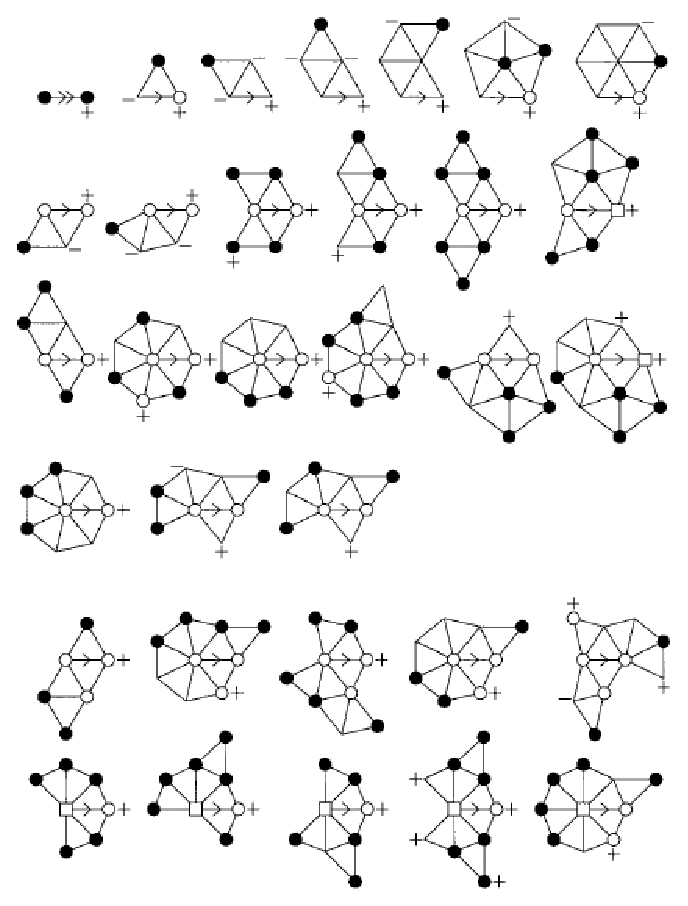
\includegraphics{seymour/regeln.eps}%
  \caption[Darstellung der 32 Regeln]{Darstellung der 32 Regeln, übernommen aus \cite{FourRSST}}
 \end{figure}

 Im weiteren Verlauf dieses Abschnitts benutzen wir $\itP$ nurnoch, um eine Menge von Flüssen zu beschreiben, die einer Regel gehorcht. Dazu ist zu bemerken, dass jeder Fluss genau einer Regel gehorcht, jedoch gibt es für einen Fluss $P$ einige wenige Darstellungen, die einer Regel folgen, deren Isomorphismus von $P$ auf $(K,r,s,t)$ aber nicht eindeutig ist -- zum Beispiel bei den Regeln 10 oder 31. In solchen Fällen zählen wir den Fluss $P$ nur ein mal zu $\itP$, da es sich bei $\itP$ nicht um eine Multimenge handelt.
 
 Flüsse, die der Regel 1 gehorchen, haben den Wert $r=2$, für alle anderen gilt $r=1$. Weiter unterscheiden sich die ersten sieben Regeln von den anderen. Folgt ein Fluss $P$ einer dieser Regeln, so gilt für die Quelle $s$ $\gamma_P(s) \in \{5,6\}$, während in allen anderen Regel für Quelle $s$ und Senke $t$ folgendes gilt: $\gamma_P(s) \in \{7,8\}$ und $\gamma_P(t) \geq 7$. Die ersten sieben Regeln folgen einer gewissen Systematik. Alle anderen Regeln wurden jedoch durch ungeordnetes Durchprobieren aufgestellt und folgen daher keinem besonderen Muster.
 
 Nun müssen wir noch zeigen, dass unsere Wahl von $\itP$ für Satz \ref{4.4} geeignet ist. Um dies zu erreichen, zerlegen wir Satz \ref{4.4} in drei Fälle, die wir Anhand des Grads der Radnabe $v$ des Wagenrads $W$ unterscheiden:
 \begin{itemize}
  \item $d_W(v) \leq 6$,
  \item $7 \leq d_W(v) \leq 11$ und 
  \item $d_W(v) \geq 12$.
 \end{itemize}
 
 Für den ersten dieser Fälle benötigen wir das folgende Lemma.
 
 \begin{lemmal}{}{4.5}
  Sei $W$ ein Wagenrad mit Radnabe $w$ mit $d_W(w) \in \{5,6\}$. Für $k = 1,\cdots,32$ seien $p_k$ und $q_k$ die Summen über die Werte $r(P)$ aller Flüsse $P$, die der Regel $k$ gehorchen und in $W$ auftreten, bei denen $w$ die Quelle bzw. Senke von $P$ ist. Angenommen, es tritt keine gute Konfiguration in $W$ auf, dann gilt:
  \begin{enumerate}[(i)]
   \item $p_1 = q_2 + q_3$
   \item $p_3 = q_4$
   \item $p_4 = q_5 + q_6$
   \item $p_5 = q_7$
  \end{enumerate}
 \end{lemmal}
 
 \begin{proof}
  Sei $X$ die Menge aller Tripel $(x,y,z)$ von Knoten, die mit $w$ benachbart sind, derart, dass sie alle unterschliedlich sind und $y$ sowohl zu $x$ als auch zu $z$ adjazent ist und $\gamma_W(x) = 5$ gilt. Setze $p_1 = \sharp X$. Sei weiter $q_2$ die Anzahl aller Tripel $(x,y,z) \in X$, für die $\gamma_W(y) \geq 7$ gilt, und $q_3$ die Menge der Tripel $(x,y,z) \in X$ mit $\gamma_W(y) \leq 6$ und $\gamma_W(z) \geq 6$. Da in $W$ nach Voraussetzung keine guten Konfigurationen auftreten, gibt es kein Tripel $(x,y,z) \in X$ mit $\gamma_W(y) \leq 6$ und $\gamma_W(z) = 5$. Somit gilt $q_2 + q_3 = \sharp X = p_1$.\\
  Für den Fall, dass $\gamma_W(w) = 5$ gilt, sind $p_3,p_4,p_5,q_4,q_5,q_6,q_7$ alle 0 und somit (ii), (iii) und (iv) wahr. Im weiteren sei also $\gamma_W(w) = 6$.\\
  Sei nun $X$ die Menge der Tripel $(x,y,z)$ von Knoten, die mit $w$ benachbart sind, derart, dass sie alle unterschliedlich sind, $y$ adjazent zu sowohl $x$ als auch $z$ ist, $\gamma_W(x) \leq 6$, $\gamma_W(y) \leq 6$ und $\gamma_W(u) = 5$ gilt, wobei $u$ der andere Knoten -- nicht $w$ -- ist, der sowohl zu $x$ als auch $y$ adjazent ist. Setze $p_3 = \sharp X$. Da nach Annahme keine gute Konfiguration in $W$ auftritt, gilt für jedes dieser Tripel $\gamma_W(z) \geq 6$. Somit gilt $q_4 = \sharp X = p_3$, was (ii) zeigt.\\
  Die Beweise für (iii) und (iv) verlaufen sehr ähnlich, weswegen hier nicht weiter darauf eingegangen wird.
 \end{proof}

  Aus \ref{4.5} leiten wir Folgendes her.

 \begin{satzl}{gute Konfiguration im Wagenrad I}{4.6}
  Sei $W$ ein Wagenrad mit $N_\itP(W) > 0$ und Radnabe $w$ mit $d_W(w) \in \{5,6\}$. Dann tritt eine gute Konfiguration in $W$ auf.
 \end{satzl}
 
 \begin{proof}
  Seien für die Radnabe $w$ die Werte $p_k$ und $q_k$ definiert für $k = 1,\cdots,32$, genau wie in \ref{4.5}.\\
  Angenommen, es trete keine gute Konfiguration in $W$ auf. Wir werden $N_\itP(W) = 0$ zeigen, was einen Widerspruch darstellt. Sei zuerst $\gamma_W(w) = 5$. Dann sind die $p_k = 0$ für $k = 2,\cdots,32$ und ebenfalls die $q_k = 0$ für $k = 4,\cdots,32$. Somit ergibt sich wegen \ref{4.5}
  \[ N_\itP(W) = 10 + p_1 - q_1 - q_2 - q_3 = 0 \]
  Sei nun $\gamma_W(w) = 6$. Dann folgt wieder aus \ref{4.5}
  \[ N_\itP(W) = p_1 + p_3 + p_4 + p_5 - q_2 - q_3 - q_4 - q_5 - q_6 - q_7 = 0\]
  In beiden Fällen erhalten wir unseren gesuchten Widerspruch durch einfaches Einsetzen.
 \end{proof}
 
 Nun wenden wir uns dem dritten Fall zu, also für Radnaben  mit Grad mindestens $12$. Dafür benötigen wir ein anderes Zwischenresultat.
 
 \begin{lemmal}{}{4.7}
  Sei $W$ ein Wagenrad mit Radnabe $w$ und sei $v$ ein zu $w$ adjazenter Knoten. Wenn keine gute Konfiguration in $W$ auftritt, ist die Summe über die $r(P)$ aller Flüsse $P \in \itP$, die in $W$ auftreten und die Quelle $v$ und Senke $w$ haben, höchstens 5.
 \end{lemmal}

 Der Beweis hierzu verwendet im wesentlichen die Annahme, dass keine gute Konfiguration auftreten darf und betrachtet für jeder der 32 Regeln die Anzahl $R_k$ der Flüsse, die in $W$ auftreten und der $k$-ten Regel folgen, sowie die Summe $R$ aller $R_k$ und zeigt, dass $R \leq 5$ gilt. Dazu unterscheidet der Beweis zwischen verschiedenen Zusammensetzungen von $R$ aus den $R_k$ für die fünf verschiedenen Fälle von Werten, di $\gamma_K(v)$ annehmen kann. Dies gestaltet sich sehr lang und trägt wenig zum Verständnis des eigentlichen Problems bei. Deshalb wird für den vollständigen Beweis auf \cite[Seite 21, Lemma 4.7]{FourRSST} verwiesen.
 
 Daraus leiten wir unser nächstes Teilresultat ab.
 
 \begin{satzl}{gute Konfiguration im Wagenrad II}{4.8}
  Sei $W$ ein Wagenrad mit $N_\itP(W) > 0$ und mit Radnabe $w$ mit $d_W(w) \geq 12$. Dann tritt in $W$ eine gute Konfiguration auf.
 \end{satzl}
 
 \begin{proof}
  Angenommen, es würde keine gute Konfiguration in $W$ auftreten. Setze $d = \gamma_W(w)$ und sei $D$ die Menge aller zu $w$ adjazenter Knoten. Für alle $v \in D$ sei $R(v)$ die Summe aller $r(P)$, wobei $P \in \itP$ ein Fluss mit Quelle $v$ und Senke $w$ ist, der in $W$ auftritt. Dann gilt nach \ref{4.7}, dass $\sum_{v \in D} R(v) \leq 5\cdot d$. Somit gilt
  \[ N_\itP(W) = 10(6-d) + \sum_{v \in V} R(v) \leq 10(6-d) + 5d = 60 - 5d \leq 0 \text{,}\]
  was ein Widerspruch ist.
 \end{proof}

 Damit sind zwei der drei Teile unseres ursprünglichen Ziels -- nämlich Satz \ref{4.4} und damit auch Satz \ref{2.3} zu zeigen -- geschafft. Damit bleibt noch die folgende Aussage.

 \begin{satzl}{gute Konfiguration im Wagenrad III}{4.9}
  Sei $W$ ein Wagenrad mit $N_\itP(W) > 0$ und mit Radnabe $w$ mit $d_W(w) \in \{7,8,9,10,11\}$. Dann tritt in $W$ eine gute Konfiguration auf.
 \end{satzl}
 
 Diesen wesentlichen Schritt führten \rsst\-\ in voller Länge aus -- insgesamt etwa 13000 Zeilen. Dazu verfassten sie den Beweis in maschinenlesbarer Form, die von Hand nachprüfbar ist. Dieses Nachprüfen ist zumindest theoretisch möglich, jedoch raten die vier Authoren wegen der schieren Länge davon ab. Stattdessen empfehlen sie, die Korrektheit des angegebenen Beweisalgorithmus mit einem anderen Computerprogramm zu verifizieren, was bereits nach damaligem Stand der Technick innerhalb weniger Minuten möglich war.

 Kombiniert man nun die Sätze \ref{4.6}, \ref{4.8} und \ref{4.9}, so erhält man die Aussage \ref{4.4}. Daraus ergibt sich dann die Korrektheit der Aussage \ref{2.3}, die diesen Abschnitt motiviert hat.
\end{section}